\documentclass[11pt,a4paper]{report}
\usepackage[textwidth=37em,vmargin=30mm]{geometry}
\usepackage{calc,xunicode,amsmath,amssymb,paralist,enumitem,tabu,booktabs,datetime2,xeCJK,xeCJKfntef,listings}
\usepackage{tocloft,fancyhdr,tcolorbox,xcolor,graphicx,eso-pic,xltxtra,xelatexemoji}

\newcommand{\envyear}[0]{2025}
\newcommand{\envdatestr}[0]{2025-10-25}
\newcommand{\envfinaldir}[0]{webdb/2025/20251025/final}

\usepackage[hidelinks]{hyperref}
\hypersetup{
    colorlinks=false,
    pdfpagemode=FullScreen,
    pdftitle={Web Digest - \envdatestr}
}

\setlength{\cftbeforechapskip}{10pt}
\renewcommand{\cftchapfont}{\rmfamily\bfseries\large\raggedright}
\setlength{\cftbeforesecskip}{2pt}
\renewcommand{\cftsecfont}{\sffamily\small\raggedright}

\setdefaultleftmargin{2em}{2em}{1em}{1em}{1em}{1em}

\usepackage{xeCJK,xeCJKfntef}
\xeCJKsetup{PunctStyle=plain,RubberPunctSkip=false,CJKglue=\strut\hskip 0pt plus 0.1em minus 0.05em,CJKecglue=\strut\hskip 0.22em plus 0.2em}
\XeTeXlinebreaklocale "zh"
\XeTeXlinebreakskip = 0pt


\setmainfont{Brygada 1918}
\setromanfont{Brygada 1918}
\setsansfont{IBM Plex Sans}
\setmonofont{JetBrains Mono NL}
\setCJKmainfont{Noto Serif CJK SC}
\setCJKromanfont{Noto Serif CJK SC}
\setCJKsansfont{Noto Sans CJK SC}
\setCJKmonofont{Noto Sans CJK SC}

\setlength{\parindent}{0pt}
\setlength{\parskip}{8pt}
\linespread{1.15}

\lstset{
	basicstyle=\ttfamily\footnotesize,
	numbersep=5pt,
	backgroundcolor=\color{black!5},
	showspaces=false,
	showstringspaces=false,
	showtabs=false,
	tabsize=2,
	captionpos=b,
	breaklines=true,
	breakatwhitespace=true,
	breakautoindent=true,
	linewidth=\textwidth
}






\newcommand{\coverpic}[2]{
    % argv: itemurl, authorname
    Cover photo by #2~~(\href{#1}{#1})
}
\newcommand{\makeheader}[0]{
    \begin{titlepage}
        % \newgeometry{hmargin=15mm,tmargin=21mm,bmargin=12mm}
        \begin{center}
            
            \rmfamily\scshape
            \fontspec{BaskervilleF}
            \fontspec{Old Standard}
            \fontsize{59pt}{70pt}\selectfont
            WEB\hfill DIGEST
            
            \vfill
            % \vskip 30pt
            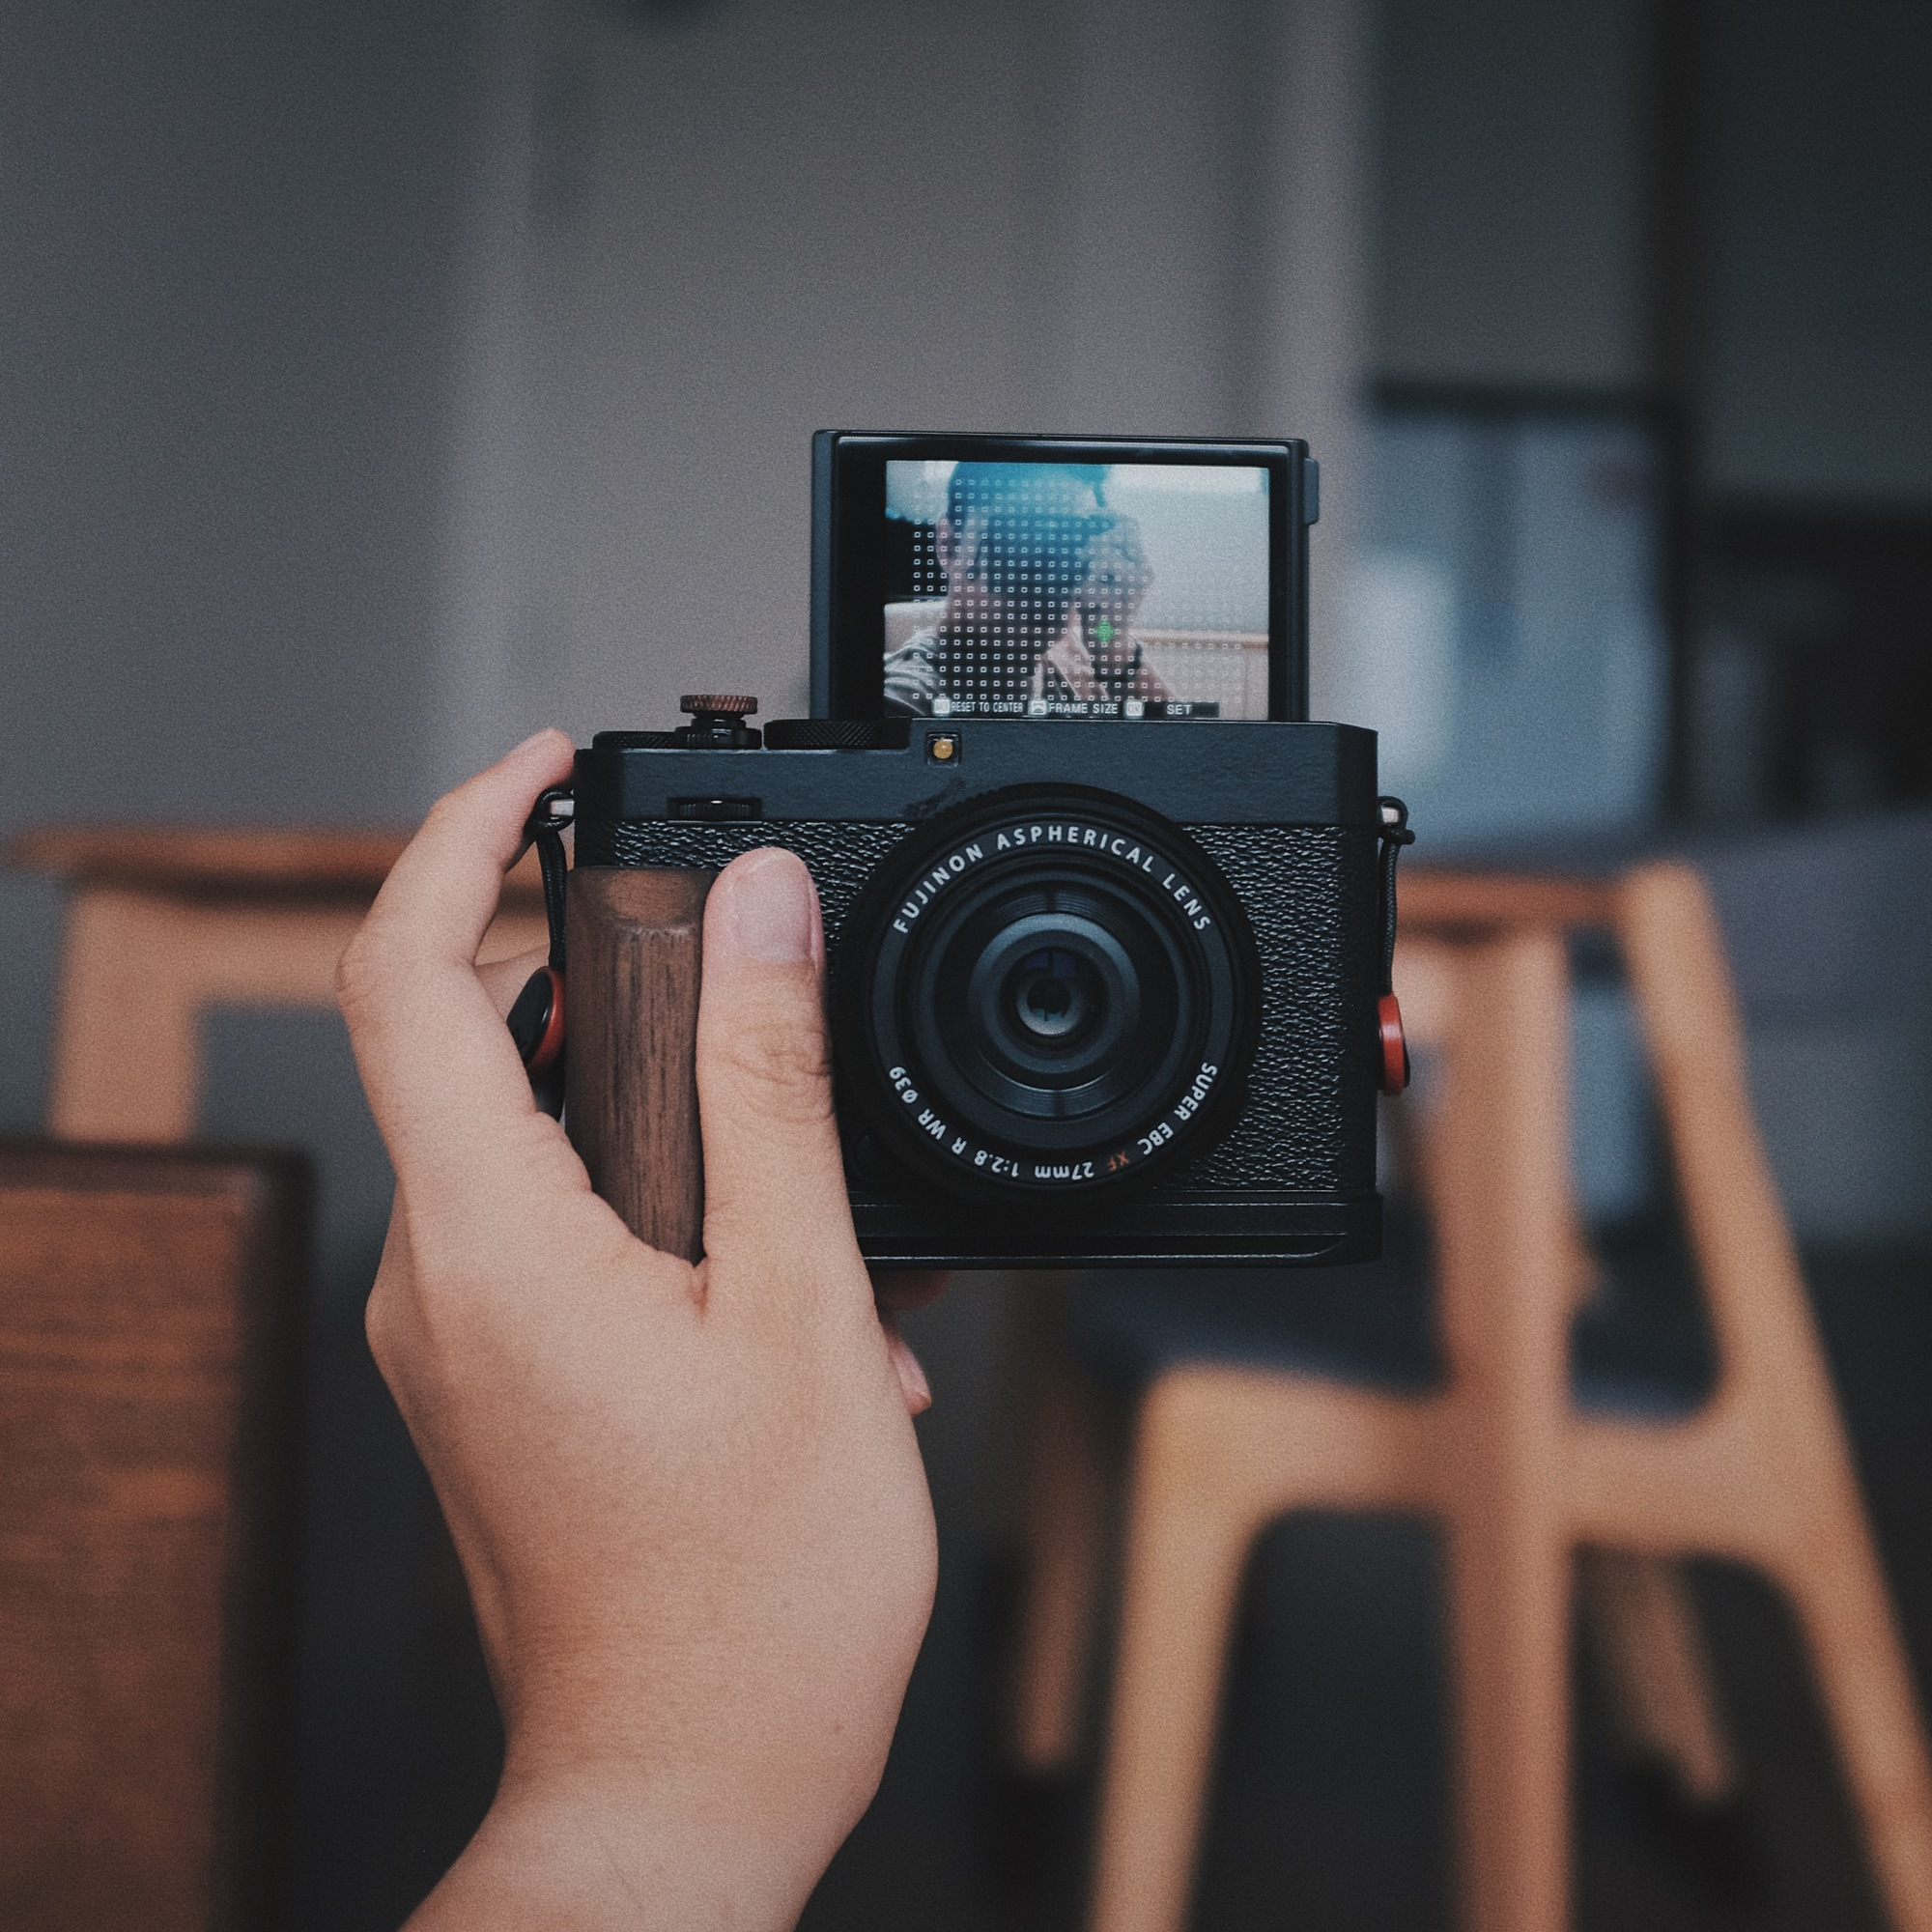
\includegraphics[width=\linewidth]{\envfinaldir/coverpic-prod.jpg}\par
            % \vskip 30pt
            \vfill

            \normalsize\rmfamily\scshape
            \copyright{} The Web Digest Project \hfill\large \envdatestr
        \end{center}
    \end{titlepage}
    % \restoregeometry
}
\newcommand{\simplehref}[1]{%
    \textcolor{blue!80!green}{\href{#1}{#1}}%
}
\renewcommand{\contentsname}{\center\Huge\sffamily\bfseries Contents\par\vskip 20pt}
\newcounter{ipartcounter}
\setcounter{ipartcounter}{0}
\newcommand{\ipart}[1]{
    % \vskip 20pt
    \clearpage
    \stepcounter{ipartcounter}
    \phantomsection
    \addcontentsline{toc}{chapter}{#1}
    % \begin{center}
    %     \Huge
    %     \sffamily\bfseries
    %     #1
    % \end{center}
    % \vskip 20pt plus 7pt
}
\newcounter{ichaptercounter}
\setcounter{ichaptercounter}{0}
\newcommand{\ichapter}[1]{
    % \vskip 20pt
    \clearpage
    \stepcounter{ichaptercounter}
    \phantomsection
    \addcontentsline{toc}{section}{\numberline{\arabic{ichaptercounter}}#1}
    \begin{center}
        \Huge
        \sffamily\bfseries
        #1
    \end{center}
    \vskip 20pt plus 7pt
}
\newcommand{\entrytitlefont}[1]{\subsection*{\raggedright\Large\sffamily\bfseries#1}}
\newcommand{\entryitemGeneric}[2]{
    % argv: title, url
    \parbox{\linewidth}{
        \entrytitlefont{#1}\par\vskip 5pt
        \footnotesize\ttfamily\mdseries
        \simplehref{#2}
    }\vskip 11pt plus 11pt minus 1pt
}
\newcommand{\entryitemGithub}[3]{
    % argv: title, url, desc
    \parbox{\linewidth}{
        \entrytitlefont{#1}\par\vskip 5pt
        \footnotesize\ttfamily\mdseries
        \simplehref{#2}\par\vskip 5pt
        \small\rmfamily\mdseries#3
    }\vskip 11pt plus 11pt minus 1pt
}
\newcommand{\entryitemAp}[3]{
    % argv: title, url, desc
    \parbox{\linewidth}{
        \entrytitlefont{#1}\par\vskip 5pt
        \footnotesize\ttfamily\mdseries
        \simplehref{#2}\par\vskip 5pt
        \small\rmfamily\mdseries#3
    }\vskip 11pt plus 11pt minus 1pt
}
\newcommand{\entryitemHackernews}[3]{
    % argv: title, hnurl, rawurl
    % \parbox{\linewidth}{
    %     \entrytitlefont{#1}\par\vskip 5pt
    %     \footnotesize\ttfamily\mdseries
    %     \simplehref{#3}\par
    %     \textcolor{black!50}{\href{#2}{#2}}
    % }\vskip 11pt plus 11pt minus 1pt
    \begin{minipage}{\linewidth}
            \entrytitlefont{#1}\par\vskip 5pt
            \footnotesize\ttfamily\mdseries
            \simplehref{#3}\par
            \textcolor{black!50}{\href{#2}{#2}}
    \end{minipage}\par\vskip 11pt plus 11pt minus 1pt
}







\begin{document}

\makeheader

\tableofcontents\clearpage




\ipart{Developers}
\ichapter{Hacker News}
\entryitemTwoLinks{The Swift SDK for Android}{https://news.ycombinator.com/item?id=45698570}{https://www.swift.org/blog/nightly-swift-sdk-for-android/}

\entryitemTwoLinks{FBI Agents Visit Anti-ICE Protester: "Your name was brought up."}{https://news.ycombinator.com/item?id=45697395}{https://www.kenklippenstein.com/p/video-fbi-agents-visit-anti-ice-protester}

\entryitemTwoLinks{Disable AI in Firefox}{https://news.ycombinator.com/item?id=45696752}{https://flamedfury.com/posts/disable-ai-in-firefox/}

\entryitemTwoLinks{First shape found that can't pass through itself}{https://news.ycombinator.com/item?id=45694856}{https://www.quantamagazine.org/first-shape-found-that-cant-pass-through-itself-20251024/}

\entryitemTwoLinks{Asahi Linux Still Working on Apple M3 Support, M1n1 Bootloader Going Rust}{https://news.ycombinator.com/item?id=45694767}{https://www.phoronix.com/news/Asahi-Linux-M3-m1n1-Update}

\entryitemTwoLinks{A sharded DuckDB on 63 nodes runs 1T row aggregation challenge in 5 sec}{https://news.ycombinator.com/item?id=45694122}{https://gizmodata.com/blog/gizmoedge-one-trillion-row-challenge}

\entryitemTwoLinks{Typst 0.14}{https://news.ycombinator.com/item?id=45693978}{https://typst.app/blog/2025/typst-0.14/}

\entryitemTwoLinks{Poker fraud used X-ray tables, high-tech glasses and NBA players}{https://news.ycombinator.com/item?id=45693599}{https://www.bbc.com/news/articles/cz6nd9wnzn6o}

\entryitemTwoLinks{Mesh2Motion – Open-source web application to animate 3D models}{https://news.ycombinator.com/item?id=45693325}{https://mesh2motion.org/}

\entryitemTwoLinks{Twake Drive – An open-source alternative to Google Drive}{https://news.ycombinator.com/item?id=45692984}{https://github.com/linagora/twake-drive}

\entryitemTwoLinks{Debian Technical Committee overrides systemd change}{https://news.ycombinator.com/item?id=45692915}{https://lwn.net/Articles/1041316/}

\entryitemTwoLinks{Interstellar Mission to a Black Hole}{https://news.ycombinator.com/item?id=45692585}{https://www.centauri-dreams.org/2025/10/23/interstellar-mission-to-a-black-hole/}

\entryitemTwoLinks{Alaska Airlines' statement on IT outage}{https://news.ycombinator.com/item?id=45691127}{https://news.alaskaair.com/on-the-record/alaska-statement-on-it-outage/}

\entryitemTwoLinks{'Attention is all you need' coauthor says he's 'sick' of transformers}{https://news.ycombinator.com/item?id=45690840}{https://venturebeat.com/ai/sakana-ais-cto-says-hes-absolutely-sick-of-transformers-the-tech-that-powers}

\entryitemTwoLinks{JupyterGIS breaks through to the next level}{https://news.ycombinator.com/item?id=45690679}{https://eo4society.esa.int/2025/10/16/jupytergis-breaks-through-to-the-next-level/}

\entryitemTwoLinks{Roc Camera}{https://news.ycombinator.com/item?id=45690251}{https://roc.camera/}

\entryitemTwoLinks{Computer science courses that don't exist, but should (2015)}{https://news.ycombinator.com/item?id=45690045}{https://prog21.dadgum.com/210.html}

\entryitemTwoLinks{Counter-Strike's player economy is in a freefall}{https://news.ycombinator.com/item?id=45689241}{https://www.polygon.com/counter-strike-cs-player-economy-multi-billion-dollar-freefall/}

\entryitemTwoLinks{React Flow, open source libraries for node-based UIs with React or Svelte}{https://news.ycombinator.com/item?id=45688836}{https://github.com/xyflow/xyflow}

\entryitemTwoLinks{Automating Algorithm Discovery: A Case Study in MoE Load Balancing}{https://news.ycombinator.com/item?id=45688236}{https://adrs-ucb.notion.site/moe-load-balancing}\ichapter{Phoronix}
\entryitemGeneric{\hskip 0pt{}OpenGL Sees New Extensions Added To The Registry}{https://www.phoronix.com/news/OpenGL-October-2025-Extensions}

\entryitemGeneric{\hskip 0pt{}The Latest Sheaves Work To Hopefully Improve Linux Performance}{https://www.phoronix.com/news/Sheaves-Replace-CPU-Slabs}

\entryitemGeneric{\hskip 0pt{}Linux Lands Fix For "Serious Performance Regression" Affecting Some Intel Chromebooks}{https://www.phoronix.com/news/Linux-618-rc3-Fix-Chromebook-PM}

\entryitemGeneric{\hskip 0pt{}AMD EPYC Turin vs. Intel Xeon 6 Granite Rapids vs. Graviton4 Benchmarks With AWS M8 Instances}{https://www.phoronix.com/review/aws-m8a-m8g-m8i-benchmarks}

\entryitemGeneric{\hskip 0pt{}Updated AMD ISP4 Driver Posted For Linux With Fixes \& Improvements}{https://www.phoronix.com/news/AMD-ISP4-Linux-Driver-v5}

\entryitemGeneric{\hskip 0pt{}Vulkan 1.4.330 Released With Five New Extensions}{https://www.phoronix.com/news/Vulkan-1.4.330-Released}

\entryitemGeneric{\hskip 0pt{}Asahi Linux Still Working On Apple M3 Support, m1n1 Bootloader Going Rust}{https://www.phoronix.com/news/Asahi-Linux-M3-m1n1-Update}

\entryitemGeneric{\hskip 0pt{}New Code Allows VCE 1.0 Video Acceleration To Work On AMDGPU Driver For GCN 1.0 GPUs}{https://www.phoronix.com/news/VCE-1.0-For-AMDGPU-Patches}

\entryitemGeneric{\hskip 0pt{}Patina 13.0 Released As Rust UEFI Firmware Implementation}{https://www.phoronix.com/news/Pantina-13.0-Rust-UEFI-Firmware}


\ipart{Developers~~~~(zh-Hans)}
\ichapter{Solidot}
\entryitemGeneric{\hskip 0pt{}2023 年海洋热浪导致佛罗里达造礁珊瑚功能性灭绝}{https://www.solidot.org/story?sid=82635}

\entryitemGeneric{\hskip 0pt{}新晋诺奖得主开发出持久性调节性T细胞}{https://www.solidot.org/story?sid=82634}

\entryitemGeneric{\hskip 0pt{}CS2 饰品暴跌市值蒸发逾 30 亿美元}{https://www.solidot.org/story?sid=82633}

\entryitemGeneric{\hskip 0pt{}亚马逊上草药类书籍可能多达 82\% 是 AI 写的}{https://www.solidot.org/story?sid=82632}

\entryitemGeneric{\hskip 0pt{}ROG Xbox Ally 的 Linux 性能超过 Windows}{https://www.solidot.org/story?sid=82631}

\entryitemGeneric{\hskip 0pt{}Django 6.0 beta 1 释出}{https://www.solidot.org/story?sid=82630}

\entryitemGeneric{\hskip 0pt{}无人机被用于投箭射杀动物}{https://www.solidot.org/story?sid=82629}

\entryitemGeneric{\hskip 0pt{}富士通推出了内置蓝光光驱的新笔电}{https://www.solidot.org/story?sid=82628}

\entryitemGeneric{\hskip 0pt{}耐药菌发展速度快于抗生素}{https://www.solidot.org/story?sid=82627}

\entryitemGeneric{\hskip 0pt{}特朗普赦免赵长鹏}{https://www.solidot.org/story?sid=82626}

\entryitemGeneric{\hskip 0pt{}中国核电总装机超 1.25 亿千瓦}{https://www.solidot.org/story?sid=82625}

\entryitemGeneric{\hskip 0pt{}天文学家在恒星宜居带发现一颗超级地球}{https://www.solidot.org/story?sid=82624}

\entryitemGeneric{\hskip 0pt{}OpenBSD 7.8 释出}{https://www.solidot.org/story?sid=82623}

\entryitemGeneric{\hskip 0pt{}Fedora 批准使用 AI 的政策}{https://www.solidot.org/story?sid=82622}

\entryitemGeneric{\hskip 0pt{}NVIDIA 中国开发者日 2025 将于11月14日在苏州举办}{https://www.solidot.org/story?sid=82620}

\entryitemGeneric{\hskip 0pt{}Google 称其量子计算机首次实现了可验证的量子优势}{https://www.solidot.org/story?sid=82619}

\entryitemGeneric{\hskip 0pt{}AWS 宕机事故导致智能床垫故障}{https://www.solidot.org/story?sid=82618}

\entryitemGeneric{\hskip 0pt{}SpaceX 禁用了缅甸电诈园区逾 2500 个Starlink 终端}{https://www.solidot.org/story?sid=82617}

\entryitemGeneric{\hskip 0pt{}Meta AI 部门裁员 600 人}{https://www.solidot.org/story?sid=82616}

\entryitemGeneric{\hskip 0pt{}VST 3 在 MIT 许可证下开源}{https://www.solidot.org/story?sid=82615}\ichapter{V2EX}
\entryitemGeneric{\hskip 0pt{}[Android] 感觉不给解 BL 锁是官方害怕售后服务成本的说法非常牵强}{https://www.v2ex.com/t/1168259}

\entryitemGeneric{\hskip 0pt{}[ WATCH] Apple Watch 2 Ultra 行货无法在美国添加 eSIM 么?}{https://www.v2ex.com/t/1168258}

\entryitemGeneric{\hskip 0pt{}[微信] 请问微信小程序的支付功能,如何监控可用性?}{https://www.v2ex.com/t/1168257}

\entryitemGeneric{\hskip 0pt{}[Android] 所谓的内置反诈是真的有这么一个对安卓定制的用户行为分析 app 吗,还是说禁止 vpn,应用黑名单,浏览器网址黑名单那些都算?}{https://www.v2ex.com/t/1168256}

\entryitemGeneric{\hskip 0pt{}[Apple] iOS26 这 TM 都是些啥啊}{https://www.v2ex.com/t/1168255}

\entryitemGeneric{\hskip 0pt{}[分享发现] 关于内置反诈}{https://www.v2ex.com/t/1168254}

\entryitemGeneric{\hskip 0pt{}[问与答] 小程序被人一比一抄袭,请问要怎么反击?}{https://www.v2ex.com/t/1168253}

\entryitemGeneric{\hskip 0pt{}[程序员] 有没有需要远程办公监控系统的}{https://www.v2ex.com/t/1168252}

\entryitemGeneric{\hskip 0pt{}[程序员] XXL-TOOL v2.3.0 发布 | Java 工具类库}{https://www.v2ex.com/t/1168251}

\entryitemGeneric{\hskip 0pt{}[奇思妙想] 感谢 v 佬做的去 sora 水印. 分享一下我为什么使用 sora}{https://www.v2ex.com/t/1168249}

\entryitemGeneric{\hskip 0pt{}[问与答] 我订阅的是 ChatGPT Pro,问模型你是哪个版本的 ChatGPT 呀?他回答我说,他是 GPT-4,我是被风控了么?}{https://www.v2ex.com/t/1168248}

\entryitemGeneric{\hskip 0pt{}[职场话题] 离职时你会把代码之类的资产打包带走么}{https://www.v2ex.com/t/1168247}

\entryitemGeneric{\hskip 0pt{}[DNS] 请教,国家自然资源部官网域名是不是在境外大多数地区都解析不出来?}{https://www.v2ex.com/t/1168245}

\entryitemGeneric{\hskip 0pt{}[买买买] 海信 E7Q 75 寸 和 索尼索尼 K-75XR50 5 系怎么选?}{https://www.v2ex.com/t/1168243}

\entryitemGeneric{\hskip 0pt{}[问与答] 2025 订阅 lightroom 的最优方案是啥}{https://www.v2ex.com/t/1168242}

\entryitemGeneric{\hskip 0pt{}[macOS] 内网前端开发需要兼容 safari, 有啥设备不带无线网卡的吗?}{https://www.v2ex.com/t/1168241}

\entryitemGeneric{\hskip 0pt{}[跑步] 震惊,髂胫束综合征居然这么痛!}{https://www.v2ex.com/t/1168240}

\entryitemGeneric{\hskip 0pt{}[奇思妙想] 饮料点评网有没有搞头}{https://www.v2ex.com/t/1168239}

\entryitemGeneric{\hskip 0pt{}[Android] 服了,手机上用了一年多的 v2rayng,习惯性打开点击连接图标,直接给我一键卸载了。}{https://www.v2ex.com/t/1168238}

\entryitemGeneric{\hskip 0pt{}[Firefox] Peek Pop 现已支持双击预览啦}{https://www.v2ex.com/t/1168237}

\entryitemGeneric{\hskip 0pt{}[问与答] ``国产安卓内置反诈后心理上就无法接受国产手机了'' 这类帖子看到过很多次了,这究竟是一种什么样的心理?}{https://www.v2ex.com/t/1168236}

\entryitemGeneric{\hskip 0pt{}[程序员] 如何解决获取 Googleplay 内购商品报错的问题}{https://www.v2ex.com/t/1168235}

\entryitemGeneric{\hskip 0pt{}[Android] 买一加国行板,刷欧/国际版 在北美地区使用, 信号好 可以接受吗?}{https://www.v2ex.com/t/1168233}

\entryitemGeneric{\hskip 0pt{}[电影] 我推荐一部安静另类的国内电影}{https://www.v2ex.com/t/1168232}

\entryitemGeneric{\hskip 0pt{}[分享创造] MOGA: 一个探索开源项目与生态可持续发展的兴趣小组 - 让开源再次伟大}{https://www.v2ex.com/t/1168230}

\entryitemGeneric{\hskip 0pt{}[宽带症候群] 问一下上海电信的如果升级了 229 的 2000M 套餐,国际精品网还能拨到 58.32 的号段吗?}{https://www.v2ex.com/t/1168229}

\entryitemGeneric{\hskip 0pt{}[问与答] 怎么让 ios app 都使用``私密查看''的方式选择照片?}{https://www.v2ex.com/t/1168227}

\entryitemGeneric{\hskip 0pt{}[酷工作] [北京] [急招] 前端、后端(Go)、大模型工程、测试}{https://www.v2ex.com/t/1168224}

\entryitemGeneric{\hskip 0pt{}[宽带症候群] 114DNS 出问题了吗?}{https://www.v2ex.com/t/1168223}

\entryitemGeneric{\hskip 0pt{}[分享创造] 自荐 | 分享一下自己建的一个 Windows 电脑软件下载网站}{https://www.v2ex.com/t/1168222}

\entryitemGeneric{\hskip 0pt{}[宽带症候群] 如果装一个电信和一个联通两条线,怎么融合比较好?用什么设备?}{https://www.v2ex.com/t/1168221}

\entryitemGeneric{\hskip 0pt{}[程序员] 帮忙看看是不是太垃圾,断断续续搞了几个月数据库监控工具,一个用户都没有}{https://www.v2ex.com/t/1168219}

\entryitemGeneric{\hskip 0pt{}[分享创造] App 开发旅程之一: 照片卡通美化工具 CatosAI}{https://www.v2ex.com/t/1168217}

\entryitemGeneric{\hskip 0pt{}[生活] 法官}{https://www.v2ex.com/t/1168216}

\entryitemGeneric{\hskip 0pt{}[投资] 刚才看到定投标普 500 和纳斯达克 100 的帖子,有一些疑问}{https://www.v2ex.com/t/1168215}

\entryitemGeneric{\hskip 0pt{}[程序员] 🌈🌈🌈 [1024,念头通达] 汇报今日收获🎉🎉🎉}{https://www.v2ex.com/t/1168214}

\entryitemGeneric{\hskip 0pt{}[Java] mysql 慢日志分析排查小工具}{https://www.v2ex.com/t/1168213}

\entryitemGeneric{\hskip 0pt{}[问与答] 方言翻译有什么好办法吗}{https://www.v2ex.com/t/1168212}

\entryitemGeneric{\hskip 0pt{}[V2EX] 网站暴涨 30 倍用户,却被国外广告平台坑了}{https://www.v2ex.com/t/1168211}

\entryitemGeneric{\hskip 0pt{}[Solana] 出现技术性双底了,可以期待一下}{https://www.v2ex.com/t/1168210}

\entryitemGeneric{\hskip 0pt{}[Apple] macOS 装 Edge 浏览器还是很难卸载吗?}{https://www.v2ex.com/t/1168209}

\entryitemGeneric{\hskip 0pt{}[Google] 被 Google One 扣了 28.99 美金,想哭,不该手贱点试用的,实际上我也没有用它这个😭, 就试用了一会会}{https://www.v2ex.com/t/1168208}

\entryitemGeneric{\hskip 0pt{}[分享创造] 上线了一个体验还不错的一站式换脸网站(赠送兑换码)}{https://www.v2ex.com/t/1168207}

\entryitemGeneric{\hskip 0pt{}[Telegram] 电报双向申诉有用吗?求申诉模版}{https://www.v2ex.com/t/1168206}

\entryitemGeneric{\hskip 0pt{}[PHP] 重造 PHP -HTTP 性能检测,新增 List<int>、HashMap<K, V>}{https://www.v2ex.com/t/1168205}

\entryitemGeneric{\hskip 0pt{}[分享发现] 1024 节日,麦当劳可以领取 29.9 元 巨无霸三件套券。}{https://www.v2ex.com/t/1168203}

\entryitemGeneric{\hskip 0pt{}[问与答] macos 的 chrome 浏览器在一些页面有奇怪的视觉效果, 这个有办法解决吗}{https://www.v2ex.com/t/1168201}

\entryitemGeneric{\hskip 0pt{}[Apple] iPhone 现在越狱后,有啥好玩的 app 么?}{https://www.v2ex.com/t/1168200}

\entryitemGeneric{\hskip 0pt{}[程序员] 为什么没有程序员 1024 相关的动图表情包之类的}{https://www.v2ex.com/t/1168199}

\entryitemGeneric{\hskip 0pt{}[问与答] 求助: iOS 上有哪些 APP 带有 Google 广告的,并且不是 Google 自家的}{https://www.v2ex.com/t/1168197}


\ipart{Generic News}







\clearpage
\leavevmode\vfill
\footnotesize

Copyright \copyright{} 2023-2025 Neruthes and other contributors.

This document is published with CC BY-NC-ND 4.0 license.

The entries listed in this newsletter may be copyrighted by their respective creators.

This newsletter is generated by the Web Digest project.

The newsletters are also delivered via Telegram channel \CJKunderline{\href{https://t.me/webdigestchannel}{https://t.me/webdigestchannel}}.\\
RSS feed is available at \CJKunderline{\href{https://webdigest.pages.dev/rss.xml}{https://webdigest.pages.dev/rss.xml}}.

This newsletter is available in PDF at
\CJKunderline{\href{https://webdigest.pages.dev/}{https://webdigest.pages.dev/}}.

The source code being used to generate this newsletter is available at\\
\CJKunderline{\href{https://github.com/neruthes/webdigest}{https://github.com/neruthes/webdigest}}.

This newsletter is also available in
\CJKunderline{\href{http://webdigest.pages.dev/readhtml/\envyear/WebDigest-20251025.html}{HTML}} and
\CJKunderline{\href{https://github.com/neruthes/webdigest/blob/master/markdown/\envyear/WebDigest-20251025.md}{Markdown}}.


\coverpic{https://unsplash.com/photos/whale-tail-emerging-from-ocean-water-with-seagulls-mt-iRSSqnfY}{James Lee}


\end{document}
